\makeatletter\let\ifGm@compatii\relax\makeatother 
\documentclass{beamer}

%-----------------------------------------------------------------------------------------

\usepackage{pgfarrows,pgfnodes,pgfautomata,pgfheaps,tikz}
\usepackage{amsmath,amssymb}
\usepackage{color}
\usepackage[latin1]{inputenc}
\usepackage{xspace}
\usepackage{graphicx}
\usepackage{graphs}
%\usepackage{listings}
\usepackage{algorithm, algpseudocode}
 
%-----------------------------------------------------------------------------------------

\usetikzlibrary{arrows,automata,shapes}
\setbeamertemplate{navigation symbols}{}
\newcommand{\redstar}{\color{red}$\bigstar$\color{black}\xspace}
\fillednodesfalse
\graphlinewidth{0.003}
\grapharrowwidth{0.4}
\grapharrowlength{0.2}
\grapharrowtype{2}
\definecolor{greenOk}{rgb}{0,.7,0} 
\definecolor{lightgray}{gray}{0.7}

%-----------------------------------------------------------------------------------------

\setbeamertemplate{background canvas}[vertical shading,bottom=red!10,top=blue!10]
%\usetheme{JuanLesPins}
\usetheme{Singapore}
\usefonttheme[onlysmall]{structurebold}
\setbeamercovered{dynamic}

%-----------------------------------------------------------------------------------------

\title[Una Metaheur�stica GRASP para Integraci�n en Grafos]{\large{Una Metaheur�stica GRASP para Integraci�n en Grafos}}
\author{Dubinsky - Massri - Asteasuain}
\institute{Depto. de Tecnolog�a y Administraci�n - Univ. Nacional de Avellaneda \\ Depto. de Matem�tica - Univ. CAECE}
\date[DLT 2003]{JAIIO-SIO \\ \footnotesize{Septiembre de 2017}}
\subject{Concurso Docente}

%-----------------------------------------------------------------------------------------


\begin{document}

\frame[plain]{\titlepage}


\begin{frame}
\frametitle{Introducci�n}
\tableofcontents[pausesections]
\end{frame}

\section{Preliminares}
\begin{frame}[t]
\frametitle{Matriz laplaciana}

\begin{block}{Definici�n}
Dado un grafo $G=(V,E)$, su \emph{matriz laplaciana} $L \in 
\mathbb{N}^{|V| \times |V|}$ se define del siguiente modo:

$$
	L_{ij} =
	\begin{cases}
	deg(v_i) & \text{si $i = j$} \\
	-1 & \text{si existe el eje $(v_i,v_j)$} \\
	0 & \text{en otro caso} 
	\end{cases}
$$

\begin{columns}[t]
	\column{.5\textwidth}
\only<2->{	
	\begin{center}
		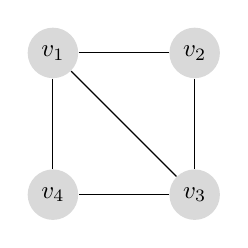
\begin{tikzpicture}[scale=.9, transform shape]
		\tikzstyle{every node} = [circle, fill=gray!30]
		\node (1) at (0, 2) {$v_1$};
		\node (2) at (2, 2) {$v_2$};
		\node (3) at (2, 0) {$v_3$};
		\node (4) at (0, 0) {$v_4$};

		\tikzstyle{every node} = [draw=none,fill=none,font=\scriptsize,midway]
		\draw [-] (1) -- (2);
		\draw [-] (1) -- (3);
		\draw [-] (1) -- (4);
		\draw [-] (2) -- (3);
		\draw [-] (3) -- (4);
		\end{tikzpicture}
	\end{center}
}
	\column{.5\textwidth}
\only<3>{
	\begin{center}	
		$L = \begin{bmatrix}
			 3 & -1 & -1 & -1  \\
			-1 &  3 & -1 &  0  \\
			-1 & -1 &  3 & -1  \\
			-1 &  0 & -1 &  3  \\
		\end{bmatrix}$
	\end{center}
}
\end{columns}

\end{block}


\end{frame}

\begin{frame}[t]
\frametitle{Matriz de incidencia dirigida}

\begin{block}{Definici�n}
Dado un grafo dirigido $G=(V,E)$, su \emph{matriz de incidencia 
dirigida} $D \in \{-1,0,1\}^{|E| \times |V|}$ es aquella tal que para 
cada eje dirigido $e_k=(v_i \rightarrow v_j)$ vale: $D_{ki}=-1$, 
$D_{kj}=1$ y vale $0$ en las dem�s entradas. Obs: $L = D^tD$
\end{block}

\begin{columns}[t]
	\column{.5\textwidth}
\only<2->{	
	\begin{center}
		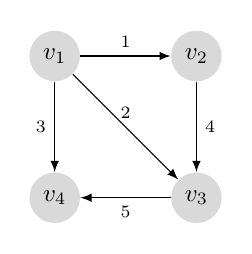
\begin{tikzpicture}[scale=.9, transform shape, >=latex]
		\tikzstyle{every node} = [circle, fill=gray!30]
		\node (1) at (0, 2) {$v_1$};
		\node (2) at (2, 2) {$v_2$};
		\node (3) at (2, 0) {$v_3$};
		\node (4) at (0, 0) {$v_4$};

		\tikzstyle{every node} = [draw=none,fill=none,font=\scriptsize,midway]
		\draw [->] (1) -- node[above] {1} (2);
		\draw [->] (1) -- node[above] {2} (3);
		\draw [->] (1) -- node[left] {3} (4);
		\draw [->] (2) -- node[right] {4} (3);
		\draw [->] (3) -- node[below] {5} (4);
		\end{tikzpicture}
	\end{center}
}
	\column{.5\textwidth}
\only<3>{
	\begin{center}	
		$D = \begin{bmatrix}
			-1 &  1 &  0 & 0  \\
			-1 &  0 &  1 & 0  \\
			-1 &  0 &  0 & 1  \\
			 0 & -1 &  1 & 0  \\
			 0 &  0 & -1 & 1  \\
		\end{bmatrix}$
	\end{center}
}
\end{columns}

\end{frame}


\begin{frame}
\frametitle{Proyecci�n ortogonal}


\end{frame}

\section{Contexto}

\begin{frame}
\frametitle{Mallas poligonales}

\begin{itemize}
	\item Grafos que modelan superficies inmersas en $\mathbb{R}^3$
	\item Los v�rtices son un muestra de los puntos de la superficie
	\item A cada v�rtice se le asocia su posicion en el espacio (ej.: 
	coordenadas cartesianas)
	\item Los ciclos simples del grafo se denominan \emph{caras}
	\item Las caras son pol�gonos convexos simples (ej.: tri�ngulos o 
	cuadrados) que modelan una peque�a parte de la superficie  aproximando 
	linealmente sus puntos interiores
\end{itemize}


\end{frame}

\begin{frame}
\frametitle{Deformaci�n de mallas poligonales}

\begin{itemize}
	\item Una \emph{deformaci�n} de una malla poligonal $S$ es un mapa 
	$d: S \rightarrow S'$ que asocia a cada punto $p \in S$ un vector de 
	desplazamiento $d(p)$.
	\item Este tipo de operaciones es frecuente en herramientas de dise�o 
	3D (ej.: arquitectura, industria, dibujos de animaci�n, etc.)
\end{itemize}

\end{frame}

\begin{frame}
\frametitle{Integraci�n de 1-formas diferenciales}

\end{frame}

\section{Problema}

\begin{frame}
\frametitle{Formulaci�n}

Problema de Minimizacion
Encontrar la mejor orientacion de los ejes
Subespacio en el que la norma de la proyeccion ortogonal del vector de pesos es m�xima
\end{frame}

\begin{frame}
\frametitle{Posibles aplicaciones}

\end{frame}

\section{Estrategia}

\begin{frame}
\frametitle{$\alpha$-norma}

Gram-Schmidt es costoso, ver costo
Estimacion de la norma: $\alpha$-norma 
�ngulos acotados entre las columnas de una matriz de incidencia dirigida

\end{frame}

\section{Implementaci�n}

\begin{frame}
\frametitle{Metaheur�sticas GRASP}

\end{frame}

\begin{frame}
\frametitle{Algoritmo}

Par�metros

\end{frame}

\begin{frame}
\frametitle{Detalles t�cnicos}

\end{frame}

\begin{frame}
\frametitle{Casos de prueba}

\end{frame}


\section{Conclusiones}
\begin{frame}
\frametitle{Conclusiones}

\end{frame}

\begin{frame}[fragile]

\begin{center}
�Preguntas?
\end{center}
\end{frame}


%----------------------------------------------------------------------------------------------------
\end{document}
